% =====================================================================
% FRQ MIRT Results  (TutorBench + TutorEval)
% File: AdaptiveTesting/Research/_paper_build/sections/41_frq_mirt_results.tex
%
% Provenance / authorship convention:
%   - Plain black text is transcribed (and lightly cleaned) from the human
%     outline PDF "CAT for Accelerated Pedagogy Benchmarking.pdf".
%   - \aiadd{...} (blue) marks additions written for this draft, cross-checked
%     against the local study data in AdaptiveTesting/Research/03_FRQ_MIRT.
%   - Fully-AI subsections end with an \aibullets{...} itemize summary.
%   - TutorEval is transcribed from the PDF ONLY (no local TutorEval data
%     exists; nothing was recomputed or supplemented).
%
% Preamble requirements (define upstream if not already present):
%   \usepackage{graphicx}   % \includegraphics
%   \usepackage{booktabs}   % \toprule \midrule \bottomrule
%   \usepackage{xcolor}     % \textcolor, \color  (for \aiadd / \aibullets)
%   \usepackage{siunitx}    % optional; not required by this file
%   Point \graphicspath to the figure source dir, or copy the basenames into
%   a local figures/ folder. The \includegraphics calls use figures/<basename>.
%
% Figure source paths (absolute), copied into ./figures/ (i.e. sections/figures/):
%   figures/tb115_recovery_scatter_correctness.png
%     <- /Users/arhant/Documents/EDLM/olmo-eval-full/AdaptiveTesting/Research/03_FRQ_MIRT/figures/tb115_recovery_scatter_correctness.png
%   figures/tb115_recovery_scatter_scaffolding.png
%     <- /Users/arhant/Documents/EDLM/olmo-eval-full/AdaptiveTesting/Research/03_FRQ_MIRT/figures/tb115_recovery_scatter_scaffolding.png
%   figures/tb115_se_reduction_curve.png
%     <- /Users/arhant/Documents/EDLM/olmo-eval-full/AdaptiveTesting/Research/03_FRQ_MIRT/figures/tb115_se_reduction_curve.png
%   figures/leaderboard_bars_correctness.png
%     <- /Users/arhant/Documents/EDLM/olmo-eval-full/AdaptiveTesting/Research/03_FRQ_MIRT/figures/leaderboard_bars_correctness.png
%
% Tables use booktabs (\toprule/\midrule/\bottomrule); ensure \usepackage{booktabs}.
% Heading level: this file opens at \section (matches sections/40_frq_judge.tex).
% If it is \input under an existing FRQ \section, demote every heading by one level.
% =====================================================================

% provenance macros (safe no-ops if already defined upstream)
\providecommand{\aiadd}[1]{\textcolor{blue}{#1}}
\providecommand{\aibullets}[1]{{\color{blue}#1}}

\section{Free-response track: MIRT results}
\label{sec:frq-mirt}

Using the criterion-level response matrix and the Q-matrix from the judge
pipeline (Section~\ref{sec:frq-judge}), we calibrate a multidimensional 2PL and
run a multidimensional CAT that selects scenarios one at a time until each skill
reaches its standard-error target.
\aiadd{TutorBench~\cite{srinivasa2025tutorbench} is the primary instrument,
calibrated on our own response data; TutorEval~\cite{chevalier2024language} is
reported from the outline only.}

\subsection{TutorBench}
\label{sec:frq-mirt-tb}

\subsubsection{Data preprocessing}
TutorBench comes with premade scenarios and rubric criteria. We ingested these
and normalized them to our own schemas, keeping the content largely intact.
Changes to scenario and question text were minor and cosmetic. Changes to
criterion text were larger: presentation criteria were normalized across
scenarios rather than left in random positions, typos were fixed, and other
deterministic corrections were applied across criteria, with some criteria
(presentation) marked optional. We then decided the Q-mapping. The initial
skills were content, diagnosis, and scaffolding. Content and diagnosis were
collapsed because of collinearity, which gives a correctness and scaffolding
pair, with presentation added as a third skill when we consider a 3-skill model.
The Q-matrix 1-values were assigned with the Q-matrix generation workflow.
\aiadd{On the 115-model matrix the 3-skill confirmatory M2PL fit gives a latent
correlation between content and diagnosis of $0.94$, which is what motivates
collapsing them into one correctness axis; the same pattern held at $N=82$.}

\subsubsection{What the skills are}
\begin{itemize}
  \item \textbf{Correctness.} Does the model give factually true information and
    diagnose the student's question accurately?
  \item \textbf{Scaffolding.} How well does the model provide a framework for
    teaching, giving hints and moving the student forward without giving away
    the answer directly?
  \item \textbf{Presentation.} How well does the model use Markdown and \LaTeX{}
    formatting, refer to the student in the second person, and follow
    convention?
\end{itemize}

\subsubsection{Choice factors}
Two settings were varied. The first is the number of skills: 1 skill
(unidimensional), 2 skills (correctness and scaffolding), or 3 skills
(correctness, scaffolding, and presentation). The second is the ability
estimator: Gaussian, batch EAP, or MWLE.

\subsubsection{Ideal calibration conditions}
The chosen configuration is 115 models in the 0.1B to 7B range, a 2-skill model
(correctness and scaffolding), and batch EAP / MWLE ability estimates. Item
selection uses the Fisher information trace rather than D-optimality.
Presentation is reported separately.
\aiadd{The 115 models are the original 82-model TutorBench calibration set plus
33 non-overlapping AWS Qwen-judge models, a clean union with zero overlaps. The
merged response matrix is 115 models by 6{,}507 criteria and is 95.1\% filled.
The definitive 2-skill bank fits 3{,}669 items over 415{,}118 observed cells,
with median discriminations of $0.98$ (correctness) and $0.80$ (scaffolding). We
fit a confirmatory M2PL by marginal maximum likelihood, with a Bock-Aitkin EM
step over a Gauss-Hermite grid and loadings masked by the Q-matrix, following
standard MIRT practice~\cite{chalmers2012mirt}.}

\subsubsection{Validation metrics}
We report the following. \emph{r} is the correlation of the CAT ability estimate
against the full-bank EAP, the reference ability of the model. \emph{Slope} is
the scale of the CAT estimate against the full bank; it catches a compressed or
stretched scale that still preserves order. In most cases we use the
out-of-sample version of these metrics, computed on models held out of the
calibration set, to show generalization. \emph{Standard error} is the per-skill
error, which the CAT reduces as it runs. Total error combines the posterior SE
(from batch EAP / MWLE) with the item-parameter uncertainty, which depends on
the number of calibration models. For reproducibility, seed stability across
different random starts was around $0.15$.

\subsubsection{Minimum-scenario stopping rule}
Table~\ref{tab:tb-minscenario} sweeps the minimum-scenario floor on the 2-skill
model (in sample). We chose a floor of 12 scenarios: the metric differences
against higher floors are negligible, and it keeps the test shorter.

\begin{table}[t]
  \centering
  \caption{TutorBench minimum-scenario floor for the stopping rule (2-skill
    model, in sample). Higher floors barely move recovery or slope, so we set
    the floor to 12.}
  \label{tab:tb-minscenario}
  \begin{tabular}{rcccc c}
    \toprule
    Min & Correctness & Scaffolding & Correctness & Scaffolding & Scenario \\
    scenarios & MWLE $r$ & MWLE $r$ & MWLE slope & MWLE slope & mean \\
    \midrule
    0  & .9815 & .9419 & 1.006 & 1.085 & 21.5 \\
    12 & .9819 & .9457 & 1.002 & 1.090 & 21.9 \\
    15 & .9822 & .9481 & 1.000 & 1.087 & 22.5 \\
    20 & .9822 & .9526 & 1.007 & 1.093 & 24.0 \\
    \bottomrule
  \end{tabular}
\end{table}

\subsubsection{Estimator comparison}
Table~\ref{tab:tb-estimator} compares Gaussian, batch EAP, and MWLE. MWLE
recovers the slope best (close to 1 on both skills), with a small cost on the
scaffolding correlation.

\begin{table}[t]
  \centering
  \caption{TutorBench estimator comparison (2-skill model). MWLE gives the
    best-scaled recovery on both axes.}
  \label{tab:tb-estimator}
  \begin{tabular}{lcccc}
    \toprule
    Estimator & Correctness slope & Correctness $r$ & Scaffolding slope & Scaffolding $r$ \\
    \midrule
    Gauss     & .644 & .921 & .875 & .903 \\
    Batch EAP & .755 & .939 & .918 & .913 \\
    MWLE      & .981 & .945 & 1.032 & .902 \\
    \bottomrule
  \end{tabular}
\end{table}

\subsubsection{One, two, or three skills}
Table~\ref{tab:tb-skills} compares the 1-skill, 2-skill, and 3-skill models. The
3-skill model raises the correctness and scaffolding correlations and adds a
presentation axis, but it reaches the precision target for only 58 of 115 models
and costs about twice as many scenarios. The 2-skill model reaches the target
for all 115 models at roughly half the length, so we keep it as the default and
report presentation separately.
\aiadd{The 3-way model comparison on the 115-model data selects the collapsed
2-skill model by AIC ($\Delta$AIC vs.\ the full 3-skill model is $+3{,}251$). In
the calibrated 2-skill bank, scaffolding correlates negatively with correctness
(latent correlation about $-0.70$): models graded more correct tend to be graded
lower on scaffolding on this bank, a pattern worth flagging.}

\begin{table}[t]
  \centering
  \caption{TutorBench skill-count comparison. Precision is the number of models
    that reach the SE target; mean scenario is the average CAT length. The
    2-skill model reaches the target for every model at about half the length of
    the 3-skill model.}
  \label{tab:tb-skills}
  \begin{tabular}{lccc c c}
    \toprule
    Model & Correctness $r$ & Scaffolding $r$ & Presentation $r$ & Precision & Mean scenario \\
    \midrule
    1 skill & .949 & n/a  & n/a  & 115/115 & 12.1 \\
    2 skill & .945 & .902 & n/a  & 115/115 & 21.9 \\
    3 skill & .969 & .916 & .965 & 58/115  & 41.2 \\
    \bottomrule
  \end{tabular}
\end{table}

\subsubsection{Recovery and parameter uncertainty}
Table~\ref{tab:tb-recovery} reports the out-of-sample MWLE recovery, slope, and
standard error for the 2-skill model. The posterior SE is the estimator error;
the total SE adds the item-parameter uncertainty on top.
Figures~\ref{fig:tb-recovery-correctness} and~\ref{fig:tb-recovery-scaffolding}
show the out-of-sample recovery scatter for each axis,
Figure~\ref{fig:tb-se} shows how the standard error falls as the CAT runs and
how the stopping target trades off against test length, and
Figure~\ref{fig:tb-leaderboard} shows the correctness leaderboard.

\begin{table}[t]
  \centering
  \caption{TutorBench recovery and standard error (2-skill model, MWLE). Total
    SE combines the posterior SE with the item-parameter uncertainty.}
  \label{tab:tb-recovery}
  \begin{tabular}{lcccc}
    \toprule
    Skill & MWLE $r$ & MWLE slope & SE posterior & SE total \\
    \midrule
    Correctness & 0.945 & 0.981 & 0.334 & 0.412 \\
    Scaffolding & 0.902 & 1.032 & 0.307 & 0.359 \\
    \bottomrule
  \end{tabular}
\end{table}

\begin{figure}[t]
  \centering
  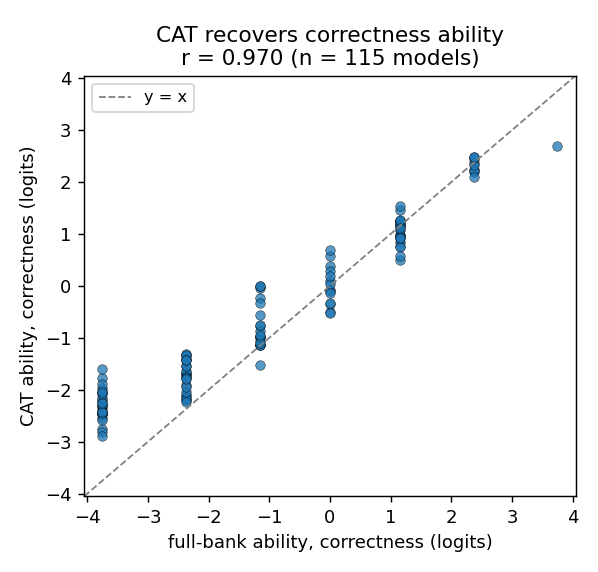
\includegraphics[width=\columnwidth]{figures/tb115_recovery_scatter_correctness.png}
  \caption{TutorBench out-of-sample recovery on the correctness axis (2-skill,
    115-model bank): CAT ability estimate against the full-bank reference.}
  \label{fig:tb-recovery-correctness}
\end{figure}

\begin{figure}[t]
  \centering
  
\includegraphics[width=\columnwidth]{figures/tb115_recovery_scatter_scaffolding.png}
  \caption{TutorBench out-of-sample recovery on the scaffolding axis (2-skill,
    115-model bank): CAT ability estimate against the full-bank reference.}
  \label{fig:tb-recovery-scaffolding}
\end{figure}

\begin{figure}[t]
  \centering
  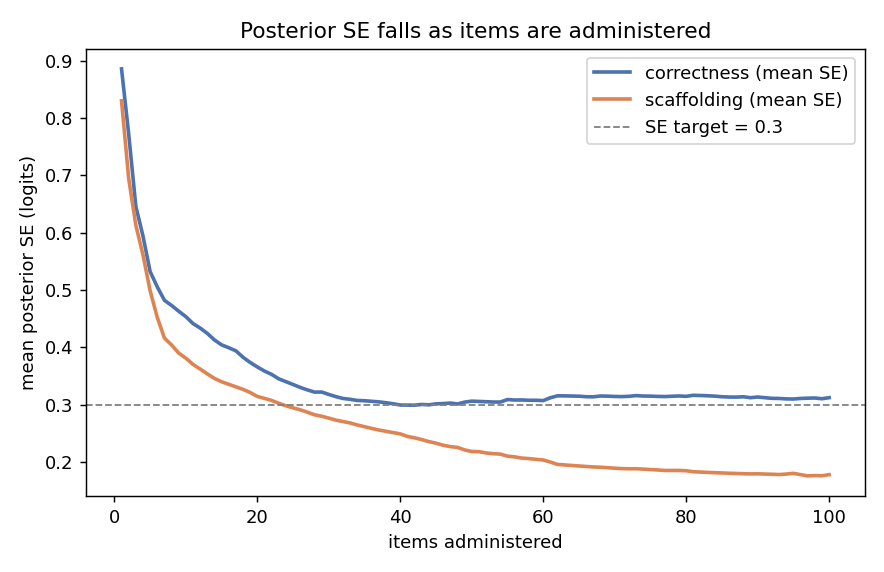
\includegraphics[width=\columnwidth]{figures/tb115_se_reduction_curve.png}
  \caption{TutorBench standard-error reduction during the CAT and the tradeoff
    between the SE target and test length (115-model bank).}
  \label{fig:tb-se}
\end{figure}

\begin{figure*}[t]
  \centering
  
\includegraphics[width=0.9\textwidth]{figures/leaderboard_bars_correctness.png}
  \caption{TutorBench correctness leaderboard from the calibrated 115-model bank.}
  \label{fig:tb-leaderboard}
\end{figure*}

\subsubsection{Final results}
With the finalized configuration, a 2-skill 2PL model (correctness and
scaffolding) calibrated on 115 models (0.1B to 7B), the adaptive test recovers
tutor ability accurately and efficiently. Using scenario-level Fisher (trace)
selection, an SE target of $0.30$, and a minimum-scenario floor of 12, all
115/115 models reach the precision target in about 22 scenarios. It recovers
correctness at an out-of-sample $r$ of $0.94$ and scaffolding at $0.91$, and it
scales properly, with a slope of $0.981$ on correctness and $1.032$ on
scaffolding. With about a 30x reduction, it nearly matches the full-bank grade in
both distribution and scale. Once item-parameter uncertainty is folded in, the
standard error runs a little high: a total SE of $0.412$ on correctness and
$0.359$ on scaffolding.
\aiadd{On the same 115-model bank, in-sample CAT recovery reaches $r=0.97$
(correctness) and $0.92$ (scaffolding), and the CAT prediction error (pIRT MAE)
is $0.022$, close to the full-bank ceiling of $0.017$. The CAT clears SE below
$0.30$ on correctness for 110 of 115 models and on scaffolding for all 115;
scaffolding alone converges in about 18 scenarios.}

\subsubsection{Limitations}
The item-parameter standard error, estimated on 115 models, is added to every
skill-ability standard error; more calibration models would bring it down from
around $0.2$ on average to something more reasonable. This effect is documented
in the psychometric literature: treating calibrated item parameters as if they
were known underestimates ability uncertainty when the calibration sample is
only moderately large~\cite{tsutakawa1990effect}, and it can make
standard-error-based stopping rules terminate variable-length CATs
early~\cite{patton2013influence}. The judge is also imperfect and does not always
agree with human graders. Finally, with only 115 models the scale is compressed
and weaker models are pulled toward the mean, which MWLE partly corrects and more
calibration models would ease further.
\aiadd{The 33 added models support this: measured with a matched
observed-information estimate at both sample sizes, the median item-loading SE
falls about 18\% from $N=82$ to $N=115$, and about 30\% on scaffolding
(Table~\ref{tab:tb-paramse}). A separate bootstrap at $N=82$ puts the median
item-loading SE at $0.41$ (correctness) and $0.60$ (scaffolding), with a median
ability-SE inflation from parameter uncertainty of about 4 to 5\%. The
cross-fold check still flags scaffolding as the weaker axis (cross-fold
discrimination $r\approx0.48$ vs.\ $0.80$ for correctness), so scaffolding is the
axis most in need of more data.}

\subsubsection{115-model calibration: cross-check against the study data}
\aiadd{This subsection is written for the draft from the local 115-model
calibration in \texttt{03\_FRQ\_MIRT}; it augments the outline rather than
transcribing it. Adding 33 models to the original 82 raises out-of-sample
recovery on both axes (most on the weaker scaffolding axis) and roughly halves
the CAT prediction error, while shrinking item-parameter uncertainty as shown in
Table~\ref{tab:tb-paramse}. The CAT length grows at $N=115$ because the merged
bank is larger and more informative and the stopping rule waits for both axes to
cross the target.}

\begin{table}[t]
  \centering
  \caption{\aiadd{Matched median item-loading standard error at $N=82$ vs.\
    $N=115$ (asymptotic observed-information estimate, same method at both sample
    sizes). More calibration models shrink parameter uncertainty, most on
    scaffolding.}}
  \label{tab:tb-paramse}
  \begin{tabular}{lccc}
    \toprule
    \aiadd{Median loading SE} & \aiadd{$N=82$} & \aiadd{$N=115$} & \aiadd{Change} \\
    \midrule
    \aiadd{All items}   & \aiadd{0.411} & \aiadd{0.337} & \aiadd{$-18\%$} \\
    \aiadd{Correctness} & \aiadd{0.419} & \aiadd{0.350} & \aiadd{$-16\%$} \\
    \aiadd{Scaffolding} & \aiadd{0.409} & \aiadd{0.287} & \aiadd{$-30\%$} \\
    \bottomrule
  \end{tabular}
\end{table}

\aibullets{%
\begin{itemize}
  \item The 115-model bank is the 82-model set plus 33 non-overlapping AWS
    Qwen-judge models (115 by 6{,}507 criteria, 95.1\% filled; 3{,}669 items
    fit).
  \item In-sample CAT recovery is $r=0.97$ (correctness) and $0.92$
    (scaffolding); pIRT MAE is $0.022$ against a full-bank ceiling of $0.017$.
  \item Going from 82 to 115 models cuts the median item-loading SE by about
    18\% overall and about 30\% on scaffolding.
  \item Scaffolding stays the weaker axis (cross-fold discrimination
    $r\approx0.48$), so it is the first place added calibration models would
    help.
\end{itemize}}

\subsection{TutorEval}
\label{sec:frq-mirt-te}

\aiadd{The TutorEval results below are transcribed from the outline PDF. There is
no local TutorEval calibration data, so nothing here was recomputed or
supplemented, and no TutorEval figures exist.}

\subsubsection{Choice factors}
We attempted both a unidimensional and a two-dimensional IRT approach. The two
skills used for the 2D model were conceptual understanding and quantitative
procedure. As with TutorBench, we compared the Gaussian, batch EAP, and MWLE
estimators.

\subsubsection{Preprocessing}
From the TutorEval dataset, the items in the \texttt{question} field are used as
scenarios. For open-book questions, the provided textbook excerpt is also
included in the scenario prompt. To get criteria for each scenario, we use the
\texttt{key points} field and split it into separate criteria (about 2 to 3
each). Some criteria were reworded to be more gradable (closer to yes/no) while
keeping the content being tested. Roughly 80 were reviewed by hand.

\subsubsection{Calibration conditions}
52 open-source models in the 0.2B to 7B parameter range were used as tutors to
calibrate the discrimination and difficulty parameters for each criterion in the
TutorEval set.

\subsubsection{CAT details}
The diagnostic finishes once the standard error is below $0.3$. Across the
selected scenarios there must be at least 15 criteria in total before the
diagnostic can end. Even if the standard error is already low enough, the test
must still reach this 15-criterion minimum.

\subsubsection{Estimator comparison}
Tables~\ref{tab:te-2d} and~\ref{tab:te-uni} report the two-dimensional and
unidimensional estimator results. Slope measures how well the CAT estimate scales
to the full bank; $r$ measures how well the CAT estimate lines up in order,
ignoring scale.

\begin{table}[t]
  \centering
  \caption{TutorEval two-dimensional estimator comparison (conceptual and
    quantitative skills). Sourced from the outline PDF.}
  \label{tab:te-2d}
  \begin{tabular}{lcccc}
    \toprule
    Estimator & Conceptual slope & Conceptual $r$ & Quantitative slope & Quantitative $r$ \\
    \midrule
    Gauss     & 0.43  & 0.8506 & 0.75  & 0.9572 \\
    Batch EAP & 0.573 & 0.9063 & 0.846 & 0.9739 \\
    MWLE      & 0.67  & 0.9122 & 0.936 & 0.9721 \\
    \bottomrule
  \end{tabular}
\end{table}

\begin{table}[t]
  \centering
  \caption{TutorEval unidimensional estimator comparison. Sourced from the
    outline PDF.}
  \label{tab:te-uni}
  \begin{tabular}{lcc}
    \toprule
    Estimator & Ability slope & Ability $r$ \\
    \midrule
    Gauss     & 0.545 & 0.9051 \\
    Batch EAP & 0.659 & 0.9349 \\
    MWLE      & 0.686 & 0.9309 \\
    \bottomrule
  \end{tabular}
\end{table}

\subsubsection{Dimensionality}
Even with the 2D approach, TutorEval essentially collapses back to
unidimensional. The two skills correlate at $0.98$. More tutor models would
likely be needed during calibration to make 2D work. Since 2D is not giving us
more information than unidimensional, we will likely stick with unidimensional for
this benchmark. Both are reported here for completeness.

\subsubsection{Reduction}
For the unidimensional model, the diagnostic uses a mean of 10.4 scenarios for
both the trace and D-optimality selection rules (about an 80x reduction), and
about 15 criteria on average, a reduction of more than 100x from the original
1786. For the 2D model, the diagnostic uses a mean of 18.3 scenarios with trace
and 27.8 scenarios with D-optimality (about a 40x reduction), and about 34
criteria on average, roughly doubling the cost.

\subsubsection{Recovery}
For the unidimensional model, MWLE recovery is $r=0.931$ (online $0.905$ / batch
$0.935$). For the 2D model, MWLE recovery is $r=0.912$ (conceptual) and $0.972$
(quantitative). MWLE has the least score shrinkage, meaning it pulls the top and
bottom scores toward the average the least.

\subsubsection{Limitations}
52 models were used during calibration and k-fold validation, which is a
relatively small number. Using more models for calibration would help strengthen
the validity of these results.
